\section{Related work}\label{sec:rel}
%In this section, we survey previous work and focus on the most relevant pieces.
%Section~\ref{sec:trajvisana} and ~\ref{sec:interactive} summarize the related works in trajectory visual analysis and interactive data visualization for large dataset, respectively.

In this part, we survey related works on \textit{trajectory visualization methods} in Section~\ref{sec:trajvisana} and \textit{interactive data visualization for large datasets} in Section~\ref{sec:interactive}, respectively.

\subsection{Trajectory Visualization Methods}\label{sec:trajvisana}
A trajectory is a sequence of spatial locations (e.g., GPS positioning results) and trajectory is the most common representation of object movements. Existing trajectory visualization methods can be classified into three categories according to the form of visualization~\cite{chen2015survey}, i.e., \textit{point-based visualization}, \textit{region-based visualization}, and \textit{line-based visualization}. We give a brief introduction to these methods and refer the interested readers to~\cite{chen2015survey} for more detailed discussions. Point-based visualization plots the locations in each trajectory independently and captures the overall spatial distribution of the moving objects. Many density-based methods, e.g., kernel density estimation, are applied in point-based visualization~\cite{liu2013vait,yang2016exploring,chae2014public,xie2008kernel, borruso2008network} to preserve the spatial distribution. Region-based visualization slices the entire region into sub-regions and visualizes the aggregated information in each sub-region~\cite{guo2009flow,wood2010visualisation,von2015mobilitygraphs}. As region-based visualization focuses on aggregated statistics, it is effective in capturing macro-patterns. In this work, we focus on line-based visualization, which uses polylines to connect the locations in each trajectory and shows the trace of object movements (see examples in Figure~\ref{fig:line}). As it preserves the continuous movement information of objects~\cite{guo2011tripvista,hurter2009fromdady}, line-based visualization is widely used in many visual analysis applications such as traffic management, urban planning, and route recommendation. However, line-based visualization is known to suffer from serve visual clutter, especially when the dataset is large. Several techniques have been proposed to alleviate visual clutter, such as clustering-based techniques~\cite{ferreira2013vector, rinzivillo2008visually, von2015mobilitygraphs} and advanced interaction techniques~\cite{kruger2013trajectorylenses, ferreira2013visual}.



\subsection{Interactive Visualization for Large Datasets}\label{sec:interactive}
%With the recent advancement of location-acquisition technology, the size of available trajectory dataset becomes extremely huge.
%For example, the operating taxis in Shenzhen generate {$\sim$}9.3GB trajectory data per day.
%Figure~\ref{fig:framework} illustrates the architecture of interactive visualization systems for large datasets,
%e.g., Spotfire~\cite{Spotfire}, Tableau~\cite{Tableau}, ATLAS~\cite{chan2008maintaining}, and Viate~\cite{yang2019vaite}.
%{It} consists of three layers: the user interface in front-end, the optimization techniques in middle-layer, and the (cloud-based) database management system in the back-end.
%{Typically, the researchers in visualization community focus on improving the effectiveness of data visualization at the front-end,
%e.g., designing novel visualization method D3~\cite{d3} to assist data analysts to obtain data insights effectively.}
%For the researchers in database community, they are working on the efficiency aspect for large data processing,
%e.g., devising big data processing system Spark~\cite{spark} for efficient query processing at back-end.
%In recent years, both visualization and database communities are dedicating to advance the techniques in interactive visual analysis for large-scale dataset,
%e.g., the optimizations in the middle-layer (see Figure~\ref{fig:framework}).
%We briefly elaborate these optimization techniques {in this section}.






Figure~\ref{fig:framework} illustrates the general architecture of interactive visualization systems,
e.g., Spotfire~\cite{Spotfire}, Tableau~\cite{Tableau}, ATLAS~\cite{chan2008maintaining}, and Viate~\cite{yang2019vaite}.
There are typically three layers: user interface in the front-end layer, optimization techniques in the middle-layer, and database management system (usually cloud-based) in the back-end layer. Researchers in the visualization community usually focus on improving the effectiveness of data visualization at the front-end, e.g., designing novel visualization methods/toolkits such as D3~\cite{d3} to enable data analysts to gain insights from data effectively. For researchers in the database community, they usually aim to improve query efficiency, e.g., devising big data processing systems such as Spark~\cite{spark} for efficient data processing at the back-end. With recent developments of location-acquisition technologies, the sizes of available trajectory datasets have become extremely large. For example, the operating taxis in Shenzhen generate {$\sim$}9.3GB trajectory data per day. However, large datasets increase visualization generation latency due to heavy data processing/graphic rendering, which harms the responsiveness of interactive visualization. Therefore, both visualization and database communities began to advance techniques in the middle-layer to reduce the visualization latency for large datasets. We briefly elaborate these techniques as follows.


\begin{figure}
	\centering
	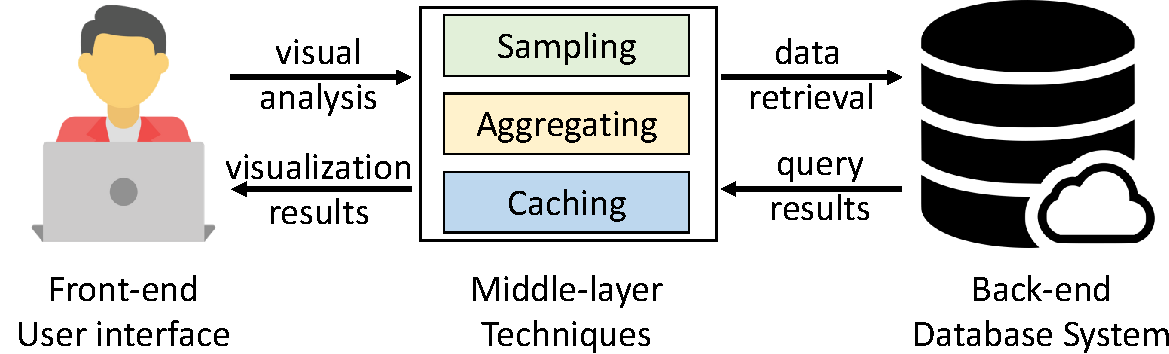
\includegraphics[width=0.40\textwidth]{pictures/framework/framework.pdf}
	\vspace{-2mm}
	\caption{System architecture for interactive visualization.} \label{fig:framework}
    \vspace{-2mm}
\end{figure}


\stitle{Aggregating-based techniques}
%{Aggregating-based techniques pre-process raw data with aggregation techniques (e.g., clustering) in the middle-layer, and yield fewer rendering objects for interactive visual analysis.}
%Returning to the trajectory visual analysis,
These works~\cite{wood2010visualisation,guo2009flow,von2015mobilitygraphs} divide the {spatial space} into basic units and visualize the aggregated information of the trajectories for each unit. For more details on aggregating-based techniques, we refer the reader to the related works~\cite{andrienko2008spatio,adrienko2010spatial}. Our problem and solutions are different from these works as we focus on visualizing the raw input data, instead of the aggregated results.
%However, aggregating-based methods will cause information loss definitely.
%For instance, the continuous spatial traces of the moving objects are always missing and the rarely appeared trajectories are easily to be ignored.






\stitle{Sampling-based techniques}
Sampling techniques are widely used in both visualization and database communities ~\cite{battle2013dynamic,rapp2019void,chen2014visual,yu2020turbocharging,park2016visualization,qin2020making,DBLP:conf/sigmod/DingHCC016,DBLP:journals/pvldb/KimBPIMR15}.

These works try to reduce the dataset to a subset with some special characters: such as the blue noise property~\ref{rapp2019void}, the multi-class property~\cite{chen2014visual} or maximize other optional user-defined quality~\cite{yu2020turbocharging}. 
The work most relevant to ours is~\cite{park2016visualization}, which is designed for scatter plots (a form of point-based visualization). It solves the problem of point overdrawing and preserves the spatial point distribution of the original dataset at the same time. The techniques in~\cite{park2016visualization} cannot be adapted to our trajectory visualization problem
as trajectory is more complex than scatter points (e.g., varying lengths, contiguous GPS points).

It's worth to mention the area of trajectory simplification~\cite{zhang2018trajectory, 2018arXiv180303550V} which is orthogonal to our proposals. Trajectory simplification tries to simplify a single trajectory by preserving the important points in a trajectory, which can be used to reduce the data size~\cite{zhang2018trajectory} or alleviate  the visual clutter~\cite{borcan2012improving, 6851202}. We refer the audience to~\cite{zhang2018trajectory} for more details. 

\stitle{Caching-based and other techniques}
%Caching is commonly used to improve the performance of large data processing system, e.g., search engine~\cite{xu2015diversified}.
Chan et al. present ATLAS~\cite{chan2008maintaining}, which utilizes caching for efficient data communication between server and client.
In addition, ATLAS also exploits a powerful multi-core server to accelerate visual analysis task processing from the middle-layer to the back-end.
Piringer et al.~\cite{piringer2009multi} propose a multi-threading architecture for interactive visual exploration,
which utilizes multi-core devices and avoids the pitfalls of multi-threading to provide quick visual feedback.
{Our} techniques in this work are orthogonal to researches in this category.

%Current advancing sampling techniques in the visualization domain are mostly
%Some works design advanced sampling algorithms to preserve the meaningful data items according to the analyzing requirement such as the multi-class data analysis and hierarchical exploration~\cite{chen2014visual}. Furthermore, to the usage of more visual channels of the points other than location such as color~\cite{chen2014visual}, size~\cite{woodruff1998constant} and opacity are discussed.
%Closely related to our work, Park et al.~\cite{park2016visualization} proposed the visualization-aware techniques for the scatter plot.
%
%In comparison with the sampling techniques for scatter plot, the trajectory sampling is more challenging because of the complexity of the trajectories~\cite{pelekis2010unsupervised}.
%
%
%Many exiting visual analytics systems leverage powerful database manage system as the backend to facilitate the fast data processing. Based on the solution proposed in ScalaR~\cite{battle2013dynamic}, a common visualization framework involving sampling technique is illustrated as Figure~\ref{fig:framework}, where a sampling layer is set between the backend and frontend. Since the sampling methods are always designed for complicated task, the algorithms may not be efficient enough to support the interactive data exploration. Thus the cache model is always implemented to save the sampling results. In our scenario, the users query large amount of data(e.g. all Shenzhen trajectories in one week) once and then conduct interactive multi-resolution exploration based on the sampled data, thus the method need to guarantee the visual quality well across different resolutions.
%
%Sampling is a delta-facto solution for the problems with big data. Target at the sampling requirement, the naive solutions such as uniform random sampling cannot generate acceptable because the serious visual information loss. In this section, we first define a loss function to evaluate the visual quality between the visualization results between whole dataset and sampled subset. Then we analyze the hardness of the problem and design algorithms for it.
%
%
%\begin{figure}[t]
%	\centering
%	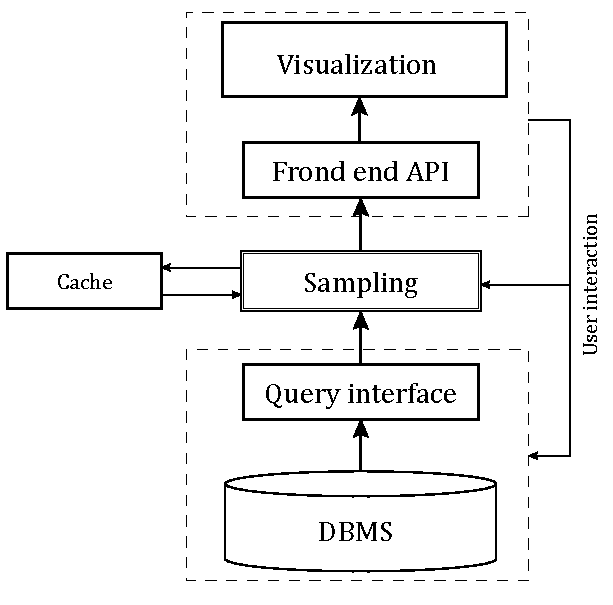
\includegraphics[width=0.3\textwidth]{pictures/framework/DBVAframework.pdf}
%	\vspace{-5mm}
%	\caption{A visualization framework involving sampling layer between the front-end and database management system.}
%	\vspace{-5mm}
%	\label{fig:framework}
%\end{figure}
%

\sstitle{Novelties of our work} To the best of our knowledge, we are the first to observe that random sampling harms visual quality for large-scale trajectory visualization and formulate the problem of quality-guaranteed sampling. To tackle this problem, we design a complete framework with quality loss function, theoretical quality loss analysis, and algorithm efficiency optimizations. The well-know visual clutter problem of trajectory visualization is also addressed naturally in our sampling framework. Extensive experimental results show that our proposals effectively maintain visual quality and reduces visualization latency at the same time.


%Our work differs from the above researches as we propose visual quality-guaranteed sampling approaches for the large-scale trajectory visualization problem,
%we demonstrate the superiority of our proposals by case-, user- and quantitative- studies in real-world dataset.
%
%Unlike existing line-based visualization techniques, we propose visual quality-guaranteed sampling approaches for line-based trajectory visualization with large-scale input data.
%To the best of our knowledge, it is the first work which offers theoretical visual quality guarantee on the sampling result for large-scale line-based trajectory visualization. 